\documentclass[../main.tex]{subfiles}

\begin{document}

\chapter{Polynomial Interpolation}\label{chap:chap17}

\begin{center}
    \Large{\textbf{CHAPTER OBJECTIVES}}
\end{center}
The primary objective of this chapter is to introduce you to polynomial interpolation.
Specific objectives and topics covered are

\begin{itemize}
    \item Recognizing that evaluating polynomial coefficients with simultaneous equations
    is an ill-conditioned problem.
    \item Knowing how to evaluate polynomial coefficients and interpolate with
    MATLAB's $polyfit$ and $polyval$ functions.
    \item Knowing how to perform an interpolation with Newton's polynomial.
    \item Knowing how to perform an interpolation with a Lagrange polynomial.
    \item Knowing how to solve an inverse interpolation problem by recasting it as a roots
    problem.
    \item Appreciating the dangers of extrapolation.
    \item Recognizing that higher-order polynomials can manifest large oscillations.
\end{itemize}

\noindent\textit{YOU'VE GOT A PROBLEM}\\
If we want to improve the velocity prediction for the free-falling bungee jumper, we might
expand our model to account for other factors beyond mass and the drag coefficient. As
was previously mentioned in Section 1.4, the drag coefficient can itself be formulated as
a function of other factors such as the area of the jumper and characteristics such as the
air's density and viscosity.
Air density and viscosity are commonly presented in tabular form as a function of
temperature. For example, Table 17.1 is reprinted from a popular fluid mechanics textbook
(White, 1999).
Suppose that you desired the density at a temperature not included in the table. In such
a case, you would have to interpolate. That is, you would have to estimate the value at the

\noindent\textit{TABLE 17.1 Density} $(\rho)$, dynamic viscosity $(\mu)$, and kinematic viscosity $(v)$ as a function of temperature $(T)$ at $1 \mathrm{~atm}$ as reported by White (1999).
\begin{center}
\begin{tabular}{rclr}
\hline $\boldsymbol{T}^{\circ} \mathbf{C}$ & $\boldsymbol{\rho}, \mathbf{k g} / \mathbf{m}^{\mathbf{3}}$ & $\boldsymbol{\mu}, \mathbf{N} \cdot \mathbf{s} / \mathbf{m}^{\mathbf{2}}$ & $\boldsymbol{v}, \mathbf{m}^{\mathbf{2}} / \mathbf{s}$ \\
\hline$-40$ & $1.52$ & $1.51 \times 10^{-5}$ & $0.99 \times 10^{-5}$ \\
0 & $1.29$ & $1.71 \times 10^{-5}$ & $1.33 \times 10^{-5}$ \\
20 & $1.20$ & $1.80 \times 10^{-5}$ & $1.50 \times 10^{-5}$ \\
50 & $1.09$ & $1.95 \times 10^{-5}$ & $1.79 \times 10^{-5}$ \\
100 & $0.946$ & $2.17 \times 10^{-5}$ & $2.30 \times 10^{-5}$ \\
150 & $0.835$ & $2.38 \times 10^{-5}$ & $2.85 \times 10^{-5}$ \\
200 & $0.746$ & $2.57 \times 10^{-5}$ & $3.45 \times 10^{-5}$ \\
250 & $0.675$ & $2.75 \times 10^{-5}$ & $4.08 \times 10^{-5}$ \\
300 & $0.616$ & $2.93 \times 10^{-5}$ & $4.75 \times 10^{-5}$ \\
400 & $0.525$ & $3.25 \times 10^{-5}$ & $6.20 \times 10^{-5}$ \\
500 & $0.457$ & $3.55 \times 10^{-5}$ & $7.77 \times 10^{-5}$ \\
\hline
\end{tabular}
\end{center}
desired temperature based on the densities that bracket it. The simplest approach is to determine the equation for the straight line connecting the two adjacent values and use this
equation to estimate the density at the desired intermediate temperature. Although such
linear interpolation is perfectly adequate in many cases, error can be introduced when the
data exhibit significant curvature. In this chapter, we will explore a number of different
approaches for obtaining adequate estimates for such situations.

\vspace{2cm}
\section{INTRODUCTION TO INTERPOLATION}

You will frequently have occasion to estimate intermediate values between precise data
points. The most common method used for this purpose is polynomial interpolation. The
general formula for an $(n - 1)$th-order polynomial can be written as

\begin{equation}
    \tag{17.1}
    f(x)=a_{1}+a_{2} x+a_{3} x^{2}+\cdots+a_{n} x^{n-1}
    \end{equation}

    For n data points, there is one and only one polynomial of order $(n - 1)$ that passes through
    all the points. For example, there is only one straight line (i.e., a first-order polynomial)
    that connects two points (Fig. 17.1a). Similarly, only one parabola connects a set of three
    points (Fig. 17.1b). Polynomial interpolation consists of determining the unique $(n - 1)$thorder polynomial that fits n data points. This polynomial then provides a formula to
    compute intermediate values.\\
    Before proceeding, we should note that MATLAB represents polynomial coefficients
    in a different manner than Eq. (17.1). Rather than using increasing powers of x, it uses decreasing powers as in

    \begin{equation}
        \tag{17.2}
        f(x)=p_{1} x^{n-1}+p_{2} x^{n-2}+\cdots+p_{n-1} x+p_{n}
        \end{equation}

        To be consistent with MATLAB, we will adopt this scheme in the following section

        \begin{figure}[H]
            \centering
            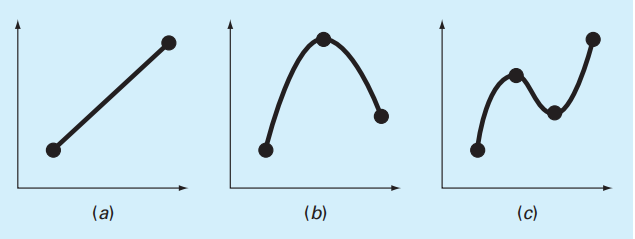
\includegraphics[scale=0.6]{fig_17_1}
           \caption{\textsf{Examples of interpolating polynomials: (a) first-order (linear) connecting two points,
           (b) second-order (quadratic or parabolic) connecting three points, and (c) third-order (cubic)
           connecting four points.}}\label{fig:fig_17_1}
        \end{figure}

        \subsection{Determining Polynomial Coefficients}
        A straightforward way for computing the coefficients of Eq. (17.2) is based on the fact that
        n data points are required to determine the n coefficients. As in the following example, this
        allows us to generate n linear algebraic equations that we can solve simultaneously for the
        coefficients.

        \begin{exmp} \textbf{First-Order Splines}
            \noindent\textit{Problem Statement.} Suppose that we want to determine the coefficients of the parabola, $f(x)=p_{1} x^{2}+p_{2} x+p_{3}$, that passes through the last three density values from Table $17.1$ :
            $$
            \begin{array}{ll}
            x_{1}=300 & f\left(x_{1}\right)=0.616 \\
            x_{2}=400 & f\left(x_{2}\right)=0.525 \\
            x_{3}=500 & f\left(x_{3}\right)=0.457
            \end{array}
            $$
            Each of these pairs can be substituted into Eq. (17.2) to yield a system of three equations:
            $$
            \begin{aligned}
            &0.616=p_{1}(300)^{2}+p_{2}(300)+p_{3} \\
            &0.525=p_{1}(400)^{2}+p_{2}(400)+p_{3} \\
            &0.457=p_{1}(500)^{2}+p_{2}(500)+p_{3}
            \end{aligned}
            $$
            or in matrix form:
            $$
            \left[\begin{array}{rrr}
            90,000 & 300 & 1 \\
            160,000 & 400 & 1 \\
            250,000 & 500 & 1
            \end{array}\right]\left\{\begin{array}{l}
            p_{1} \\
            p_{2} \\
            p_{3}
            \end{array}\right\}=\left\{\begin{array}{l}
            0.616 \\
            0.525 \\
            0.457
            \end{array}\right\}
            $$
            Thus, the problem reduces to solving three simultaneous linear algebraic equations for the three unknown coefficients. A simple MATLAB session can be used to obtain the
            \\\noindent \textbf{Solution.}
            \begin{lstlisting}[numbers=none]
>> format long
>> A = [90000 300 1;160000 400 1;250000 500 1];
>> b = [0.616 0.525 0.457];
>> p = A\b
p =
0.00000115000000
-0.00171500000000
1.02700000000000
            \end{lstlisting}

        Thus, the parabola that passes exactly through the three points is
        $$
        f(x)=0.00000115 x^{2}-0.001715 x+1.027
        $$
        This polynomial then provides a means to determine intermediate points. For example, the value of density at a temperature of $350^{\circ} \mathrm{C}$ can be calculated as
        $$
        f(350)=0.00000115(350)^{2}-0.001715(350)+1.027=0.567625
        $$
        
        \end{exmp}

        Although the approach in Example $17.1$ provides an easy way to perform interpolation, it has a serious deficiency. To understand this flaw, notice that the coefficient matrix in Example $17.1$ has a decided structure. This can be seen clearly by expressing it in general terms:
        $$
        \left[\begin{array}{lll}
        x_{1}^{2} & x_{1} & 1 \\
        x_{2}^{2} & x_{2} & 1 \\
        x_{3}^{2} & x_{3} & 1
        \end{array}\right]\left\{\begin{array}{l}
        p_{1} \\
        p_{2} \\
        p_{3}
        \end{array}\right\}=\left\{\begin{array}{l}
        f\left(x_{1}\right) \\
        f\left(x_{2}\right) \\
        f\left(x_{3}\right)
        \end{array}\right\}
        $$
    
        Coefficient matrices of this form are referred to as Vandermonde matrices. Such matrices are very ill-conditioned. That is, their solutions are very sensitive to round-off errors.
This can be illustrated by using MATLAB to compute the condition number for the coefficient matrix from Example 17.1 as

\begin{lstlisting}[numbers=none]
>> cond(A)
ans =
    5.8932e+006
\end{lstlisting}
This condition number, which is quite large for a 3 x 3 matrix, implies that about six digits
of the solution would be questionable. The ill-conditioning becomes even worse as the
number of simultaneous equations becomes larger.\\
As a consequence, there are alternative approaches that do not manifest this shortcoming. In this chapter, we will also describe two alternatives that are well-suited for
computer implementation: the Newton and the Lagrange polynomials. Before doing this,
however, we will first briefly review how the coefficients of the interpolating polynomial
can be estimated directly with MATLAB's built-in functions.

\subsection{MATLAB Functions: polyfit and polyval}
Recall from Section 14.5.2, that the $polyfit$ function can be used to perform polynomial
regression. In such applications, the number of data points is greater than the number of
coefficients being estimated. Consequently, the least-squares fit line does not necessarily
pass through any of the points, but rather follows the general trend of the data.\\
For the case where the number of data points equals the number of coefficients, $polyfit$ performs interpolation. That is, it returns the coefficients of the polynomial that pass
directly through the data points. For example, it can be used to determine the coefficients
of the parabola that passes through the last three density values from Table 17.1:

\begin{lstlisting}[numbers=none]
    >> format long
    >> T = [300 400 500];
    >> density = [0.616 0.525 0.457];
    >> p = polyfit(T,density,2)
    p =
        0.00000115000000 -0.00171500000000 1.02700000000000
\end{lstlisting}
We can then use the $polyval$ function to perform an interpolation as in

\begin{lstlisting}[numbers=none]
    >> d = polyval(p,350)
    d =
        0.56762500000000
\end{lstlisting}
These results agree with those obtained previously in Example 17.1 with simultaneous equations.

\section{NEWTON INTERPOLATING POLYNOMIAL}

There are a variety of alternative forms for expressing an interpolating polynomial beyond
the familiar format of Eq. (17.2). Newton's interpolating polynomial is among the most
popular and useful forms. Before presenting the general equation, we will introduce the
first- and second-order versions because of their simple visual interpretation.

\subsection{Linear Interpolation}

The simplest form of interpolation is to connect two data points with a straight line. This
technique, called linear interpolation, is depicted graphically in Fig. 17.2. Using similar
triangles,

\begin{equation}
    \tag{17.4}
\frac{f_{1}(x)-f\left(x_{1}\right)}{x-x_{1}}=\frac{f\left(x_{2}\right)-f\left(x_{1}\right)}{x_{2}-x_{1}}
\end{equation}
which can be rearranged to yield
\begin{equation}
    \tag{17.5}
f_{1}(x)=f\left(x_{1}\right)+\frac{f\left(x_{2}\right)-f\left(x_{1}\right)}{x_{2}-x_{1}}\left(x-x_{1}\right)
\end{equation}
which is the Newton linear-interpolation formula. The notation $f\textsubscript{1}(x)$ designates that this
is a first-order interpolating polynomial. Notice that besides representing the slope of the
line connecting the points, the term $[ f\textsubscript{1} (x\textsubscript{2}) - f (x\textsubscript{1})]/(x\textsubscript{2} - x\textsubscript{1})$ is a finite-difference

\begin{figure}[H]
    \centering
    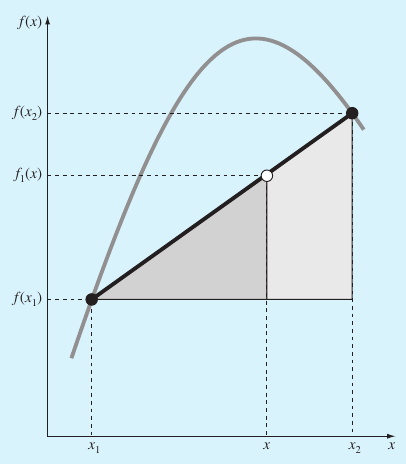
\includegraphics[scale=0.6]{fig_17_2}
   \caption{\textsf{Graphical depiction of linear interpolation. The shaded areas indicate the similar triangles used
   to derive the Newton linear-interpolation formula [Eq. (17.5)].}}\label{fig:fig_17_2}
\end{figure}

approximation of the first derivative [recall Eq. (4.20)]. In general, the smaller the interval
between the data points, the better the approximation. This is due to the fact that, as the
interval decreases, a continuous function will be better approximated by a straight line.
This characteristic is demonstrated in the following example.
\begin{exmp} \textbf{Linear Interpolation}
    \noindent\textit{Problem Statement.}Estimate the natural logarithm of 2 using linear interpolation. First,
    perform the computation by interpolating between ln 1 = 0 and ln 6 = 1.791759. Then,
    repeat the procedure, but use a smaller interval from ln 1 to ln 4 (1.386294). Note that the
    true value of ln 2 is 0.6931472.
    \noindent \textbf{Solution.} We use Eq. (17.5) from $x_{1}=1$ to $x_{2}=6$ to give
    $$
    f_{1}(2)=0+\frac{1.791759-0}{6-1}(2-1)=0.3583519
    $$
    which represents an error of $\varepsilon_{t}=48.3 \%$. Using the smaller interval from $x_{1}=1$ to $x_{2}=4$ yields
    $$
    f_{1}(2)=0+\frac{1.386294-0}{4-1}(2-1)=0.4620981
    $$

    \begin{figure}[H]
        \centering
        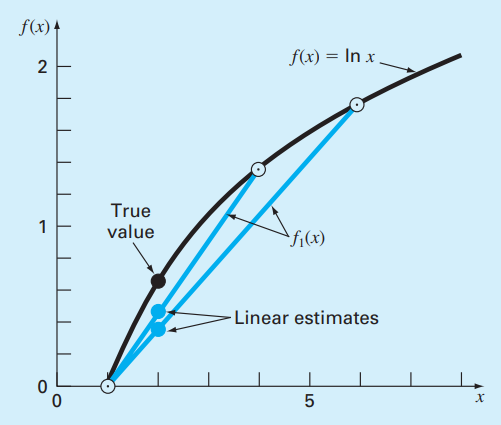
\includegraphics[scale=0.6]{fig_17_3}
       \caption{\textsf{Two linear interpolations to estimate ln 2. Note how the smaller interval provides a better
       estimate.}}\label{fig:fig_17_3}
    \end{figure}
    Thus, using the shorter interval reduces the percent relative error to $\epsilon\textsubscript{t} = 33.3\%{}$. Both
    interpolations are shown in Fig. 17.3, along with the true function.

\end{exmp}

\subsection{Quadratic Interpolation}
The error in Example 17.2 resulted from approximating a curve with a straight line. Consequently, a strategy for improving the estimate is to introduce some curvature into the line
connecting the points. If three data points are available, this can be accomplished with a
second-order polynomial (also called a quadratic polynomial or a parabola). A particularly
convenient form for this purpose is

\begin{equation}
    \tag{17.6}
    f_{2}(x)=b_{1}+b_{2}\left(x-x_{1}\right)+b_{3}\left(x-x_{1}\right)\left(x-x_{2}\right)
\end{equation}
A simple procedure can be used to determine the values of the coefficients. For $b_{1}$, Eq. (17.6) with $x=x_{1}$ can be used to compute
\begin{equation}
    \tag{17.7}
b_{1}=f\left(x_{1}\right)
\end{equation}
Equation (17.7) can be substituted into Eq. (17.6), which can be evaluated at $x=x_{2}$ for
\begin{equation}
    \tag{17.8}
b_{2}=\frac{f\left(x_{2}\right)-f\left(x_{1}\right)}{x_{2}-x_{1}}
\end{equation}
Finally, Eqs. (17.7) and (17.8) can be substituted into Eq. (17.6), which can be evaluated at $x=x_{3}$ and solved (after some algebraic manipulations) for
\begin{equation}
    \tag{17.9}
b_{3}=\frac{\frac{f\left(x_{3}\right)-f\left(x_{2}\right)}{x_{3}-x_{2}}-\frac{f\left(x_{2}\right)-f\left(x_{1}\right)}{x_{2}-x_{1}}}{x_{3}-x_{1}}
\end{equation}
Notice that, as was the case with linear interpolation, b2 still represents the slope of the
line connecting points x1 and x2. Thus, the first two terms of Eq. (17.6) are equivalent to
linear interpolation between x1 and x2, as specified previously in Eq. (17.5). The last term,
$b\textsubscript{3}(x - x\textsubscript{1})(x - x\textsubscript{2})$, introduces the second-order curvature into the formula.\\
Before illustrating how to use Eq. (17.6), we should examine the form of the coefficient $b\textsubscript{3}$. It is very similar to the finite-difference approximation of the second derivative
introduced previously in Eq. (4.27). Thus, Eq. (17.6) is beginning to manifest a structure
that is very similar to the Taylor series expansion. That is, terms are added sequentially to
capture increasingly higher-order curvature. 

\begin{exmp} \textbf{Quadratic Interpolation}
    \noindent\textit{Problem Statement.} Employ a second-order Newton polynomial to estimate ln 2 with
    the same three points used in Example 17.2:
    $$
\begin{array}{ll}
x_{1}=1 & f\left(x_{1}\right)=0 \\
x_{2}=4 & f\left(x_{2}\right)=1.386294 \\
x_{3}=6 & f\left(x_{3}\right)=1.791759
\end{array}
$$
    \noindent \textbf{Solution.} Applying Eq. (17.7) yields
    $$
    b_{1}=0
    $$
    Equation (17.8) gives
    $$
    b_{2}=\frac{1.386294-0}{4-1}=0.4620981
    $$

    \begin{figure}[H]
        \centering
        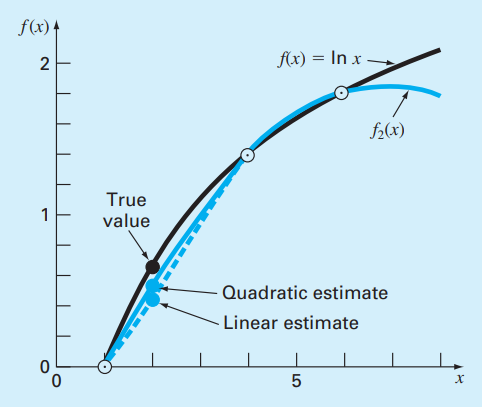
\includegraphics[scale=0.6]{fig_17_4}
       \caption{\textsf{The use of quadratic interpolation to estimate ln 2. The linear interpolation from x = 1 to 4 is
       also included for comparison.}}\label{fig:fig_17_4}
    \end{figure}
    and Eq. (17.9) yields
    $$
    b_{3}=\frac{\frac{1.791759-1.386294}{6-4}-0.4620981}{6-1}=-0.0518731
    $$
    Substituting these values into Eq. (17.6) yields the quadratic formula
    $$
    f_{2}(x)=0+0.4620981(x-1)-0.0518731(x-1)(x-4)
    $$
    which can be evaluated at $x=2$ for $f_{2}(2)=0.5658444$, which represents a relative error of $\varepsilon_{t}=18.4 \%$. Thus, the curvature introduced by the quadratic formula (Fig. 17.4) improves the interpolation compared with the result obtained using straight lines in Example 17.2 and Fig. 17.3.


\end{exmp}

\subsection{General Form of Newton's Interpolating Polynomials}
The preceding analysis can be generalized to fit an $(n - 1)$th-order polynomial to n data
points. The $(n - 1)$th-order polynomial is

\begin{equation}
    \tag{17.10}
f_{n-1}(x)=b_{1}+b_{2}\left(x-x_{1}\right)+\cdots+b_{n}\left(x-x_{1}\right)\left(x-x_{2}\right) \cdots\left(x-x_{n-1}\right)
\end{equation}
As was done previously with linear and quadratic interpolation, data points can be used to evaluate the coefficients $b_{1}, b_{2}, \ldots, b_{n}$. For an $(n-1)$ th-order polynomial, $n$ data points are required: $\left[x_{1}, f\left(x_{1}\right)\right],\left[x_{2}, f\left(x_{2}\right)\right], \ldots,\left[x_{n}, f\left(x_{n}\right)\right]$. We use these data points and the following equations to evaluate the coefficients:

\begin{equation}
    \tag{17.11}
b_{1} =f\left(x_{1}\right)
\end{equation}
\begin{equation}
    \tag{17.12}
b_{2} =f\left[x_{2}, x_{1}\right]
\end{equation}
\begin{equation}
    \tag{17.13}
b_{3} =f\left[x_{3}, x_{2}, x_{1}\right]
\end{equation}

$$\vdots$$

\begin{equation}
    \tag{17.14}
b_{n} =f\left[x_{n}, x_{n-1}, \ldots, x_{2}, x_{1}\right]
\end{equation}

where the bracketed function evaluations are finite divided differences. For example, the first finite divided difference is represented generally as
\begin{equation}
    \tag{17.15}
f\left[x_{i}, x_{j}\right]=\frac{f\left(x_{i}\right)-f\left(x_{j}\right)}{x_{i}-x_{j}}
\end{equation}
The second finite divided difference, which represents the difference of two first divided differences, is expressed generally as
\begin{equation}
    \tag{17.16}
f\left[x_{i}, x_{j}, x_{k}\right]=\frac{f\left[x_{i}, x_{j}\right]-f\left[x_{j}, x_{k}\right]}{x_{i}-x_{k}}
\end{equation}
Similarly, the $n$th finite divided difference is
\begin{equation}
    \tag{17.17}
f\left[x_{n}, x_{n-1}, \ldots, x_{2}, x_{1}\right]=\frac{f\left[x_{n}, x_{n-1}, \ldots, x_{2}\right]-f\left[x_{n-1}, x_{n-2}, \ldots, x_{1}\right]}{x_{n}-x_{1}}
\end{equation}

\begin{figure}[H]
    \centering
    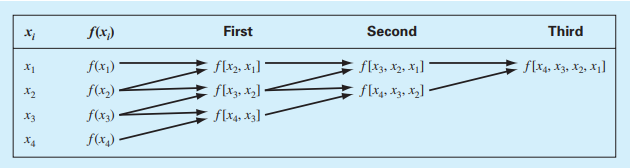
\includegraphics[scale=0.8]{fig_17_5}
   \caption{\textsf{Graphical depiction of the recursive nature of finite divided differences. This representation is
   referred to as a divided difference table.}}\label{fig:fig_17_5}
\end{figure}
These differences can be used to evaluate the coefficients in Eqs. (17.11) through (17.14),
which can then be substituted into Eq. (17.10) to yield the general form of Newton's interpolating polynomial:

\begin{equation}
    \tag{17.18}
    \begin{aligned}
    f_{n-1}(x)=& f\left(x_{1}\right)+\left(x-x_{1}\right) f\left[x_{2}, x_{1}\right]+\left(x-x_{1}\right)\left(x-x_{2}\right) f\left[x_{3}, x_{2}, x_{1}\right] \\
    &+\cdots+\left(x-x_{1}\right)\left(x-x_{2}\right) \cdots\left(x-x_{n-1}\right) f\left[x_{n}, x_{n-1}, \ldots, x_{2}, x_{1}\right]
    \end{aligned}
    \end{equation}
    We should note that it is not necessary that the data points used in Eq. (17.18) be
    equally spaced or that the abscissa values necessarily be in ascending order, as illustrated
    in the following example. However, the points should be ordered so that they are centered
    around and as close as possible to the unknown. Also, notice how Eqs. (17.15) through
    (17.17) are recursive—that is, higher-order differences are computed by taking differences
    of lower-order differences (Fig. 17.5). This property will be exploited when we develop an
    efficient M-file to implement the method.

    \begin{exmp} \textbf{Newton Interpolating Polynomial}
        \noindent\textit{Problem Statement.}In Example 17.3, data points at $x\textsubscript{1} = 1$, $x\textsubscript{2} = 4$, and $x\textsubscript{3} = 6$ were
        used to estimate ln 2 with a parabola. Now, adding a fourth point $[x\textsubscript{4} = 5$; $f (x\textsubscript{4}) = 1.609438]$, estimate ln 2 with a third-order Newton's interpolating polynomial.\\
        \noindent \textbf{Solution.} The third-order polynomial, Eq. (17.10) with $n=4$, is
        $$
        f_{3}(x)=b_{1}+b_{2}\left(x-x_{1}\right)+b_{3}\left(x-x_{1}\right)\left(x-x_{2}\right)+b_{4}\left(x-x_{1}\right)\left(x-x_{2}\right)\left(x-x_{3}\right)
        $$
        The first divided differences for the problem are [Eq. (17.15)]
        $$
        \begin{aligned}
        f\left[x_{2}, x_{1}\right] &=\frac{1.386294-0}{4-1}=0.4620981 \\
        f\left[x_{3}, x_{2}\right] &=\frac{1.791759-1.386294}{6-4}=0.2027326 \\
        f\left[x_{4}, x_{3}\right] &=\frac{1.609438-1.791759}{5-6}=0.1823216
        \end{aligned}
        $$
        The second divided differences are [Eq. (17.16)]
$$
\begin{aligned}
&f\left[x_{3}, x_{2}, x_{1}\right]=\frac{0.2027326-0.4620981}{6-1}=-0.05187311 \\
&f\left[x_{4}, x_{3}, x_{2}\right]=\frac{0.1823216-0.2027326}{5-4}=-0.02041100
\end{aligned}
$$
The third divided difference is [Eq. (17.17) with $n=4$ ]
$$
f\left[x_{4}, x_{3}, x_{2}, x_{1}\right]=\frac{-0.02041100-(-0.05187311)}{5-1}=0.007865529
$$
Thus, the divided difference table is
\begin{center}
\begin{tabular}{ccccc}
\hline $\boldsymbol{x}_{\boldsymbol{i}}$ & $\boldsymbol{f}\left(\boldsymbol{x}_{\boldsymbol{i}}\right)$ & First & Second & Third \\
\hline 1 & 0 & $0.4620981$ & $-0.05187311$ & $0.007865529$ \\
4 & $1.386294$ & $0.2027326$ & $-0.02041100$ & \\
6 & $1.791759$ & $0.1823216$ & & \\
5 & $1.609438$ & & & \\
\hline
\end{tabular}
\end{center}
The results for $f\left(x_{1}\right), f\left[x_{2}, x_{1}\right], f\left[x_{3}, x_{2}, x_{1}\right]$, and $f\left[x_{4}, x_{3}, x_{2}, x_{1}\right]$ represent the coefficients $b_{1}, b_{2}, b_{3}$, and $b_{4}$, respectively, of Eq. (17.10). Thus, the interpolating cubic is
$$
\begin{aligned}
f_{3}(x)=& 0+0.4620981(x-1)-0.05187311(x-1)(x-4) \\
&+0.007865529(x-1)(x-4)(x-6)
\end{aligned}
$$
which can be used to evaluate $f_{3}(2)=0.6287686$, which represents a relative error of $\varepsilon_{t}=9.3 \%$. The complete cubic polynomial is shown in Fig. 17.6.
    \end{exmp}

    \begin{figure}[H]
        \centering
        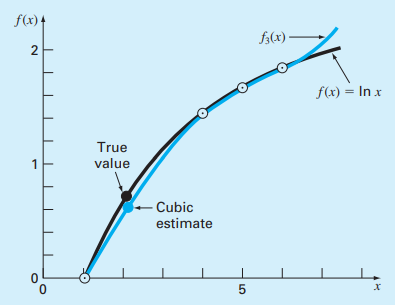
\includegraphics[scale=0.8]{fig_17_6}
       \caption{\textsf{The use of cubic interpolation to estimate ln 2.}}\label{fig:fig_17_6}
    \end{figure}

    \subsection{MATLAB M-file: Newtint}
    It is straightforward to develop an M-file to implement Newton interpolation.As in Fig. 17.7,
    the first step is to compute the finite divided differences and store them in an array. The differences are then used in conjunction with Eq. (17.18) to perform the interpolation.\\
    An example of a session using the function would be to duplicate the calculation we
    just performed in Example 17.3:
    
    \begin{lstlisting}[numbers=none]
>> format long
>> x = [1 4 6 5]';
    \end{lstlisting}
    
    \begin{figure}[H]
        \centering
        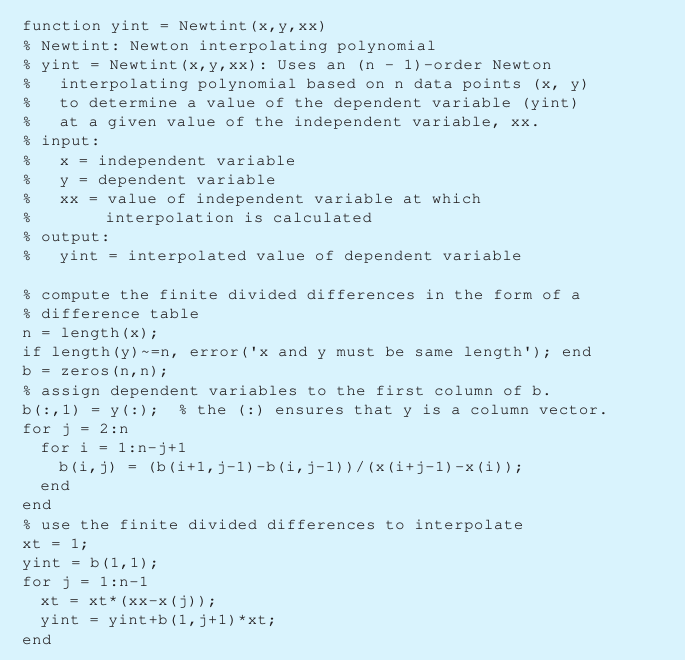
\includegraphics[scale=0.8]{fig_17_7}
       \caption{\textsf{An M-file to implement Newton interpolation.}}\label{fig:fig_17_7}
    \end{figure}

    \begin{lstlisting}[numbers=none]
        function yint = Newtint(x,y,xx)
        % Newtint: Newton interpolating polynomial
        % yint = Newtint(x,y,xx): Uses an (n - 1)-order Newton
        %   interpolating polynomial based on n data points (x, y)
        %   to determine a value of the dependent variable (yint)
        %   at a given value of the independent variable, xx.
        %  input:
        %   x = independent variable
        %   y = dependent variable
        %   xx = value of independent variable at which
        %       interpolation is calculated
        % output:
        %   yint = interpolated value of dependent variable

        % compute the finite divided differences in the form of a
        % difference table
        n = length(x);
        if length(y)~=n, error('x and y must be same length'); end
        b = zeros(n,n);
        % assign dependent variables to the first column of b.
        b(:,1) = y(:); % the (:) ensures that y is a column vector.
        for j = 2:n
            for i = 1:n-j+1
                b(i,j) = (b(i+1,j-1)-b(i,j-1))/(x(i+j-1)-x(i));
            end
        end
        % use the finite divided differences to interpolate
        xt = 1;
        yint = b(1,1);
        for j = 1:n-1
            xt = xt*(xx-x(j));
            yint = yint+b(1,j+1)*xt;
        end



        >> y = log(x);
        >> Newtint(x,y,2)

        ans =
            0.62876857890841
    \end{lstlisting}


    \section{LAGRANGE INTERPOLATING POLYNOMIAL}
    Suppose we formulate a linear interpolating polynomial as the weighted average of the two
    values that we are connecting by a straight line:
    \begin{equation}
        \tag{17.19}
    f(x)=L_{1} f\left(x_{1}\right)+L_{2} f\left(x_{2}\right)
\end{equation}
    where the $L$ 's are the weighting coefficients. It is logical that the first weighting coefficient is the straight line that is equal to 1 at $x_{1}$ and 0 at $x_{2}$ :
    $$
    L_{1}=\frac{x-x_{2}}{x_{1}-x_{2}}
    $$
    Similarly, the second coefficient is the straight line that is equal to 1 at $x_{2}$ and 0 at $x_{1}$ :
    $$
    L_{2}=\frac{x-x_{1}}{x_{2}-x_{1}}
    $$
    Substituting these coefficients into Eq. $17.19$ yields the straight line that connects the points (Fig. 17.8):
    \begin{equation}
        \tag{17.20}
    f_{1}(x)=\frac{x-x_{2}}{x_{1}-x_{2}} f\left(x_{1}\right)+\frac{x-x_{1}}{x_{2}-x_{1}} f\left(x_{2}\right)
\end{equation}
    where the nomenclature $f_{1}(x)$ designates that this is a first-order polynomial. Equation (17.20) is referred to as the linear Lagrange interpolating polynomial.
    
    The same strategy can be employed to fit a parabola through three points. For this case three parabolas would be used with each one passing through one of the points and equaling zero at the other two. Their sum would then represent the unique parabola that connects the three points. Such a second-order Lagrange interpolating polynomial can be written as
    \begin{equation}
        \tag{17.21}
    \begin{aligned}
    f_{2}(x)=& \frac{\left(x-x_{2}\right)\left(x-x_{3}\right)}{\left(x_{1}-x_{2}\right)\left(x_{1}-x_{3}\right)} f\left(x_{1}\right)+\frac{\left(x-x_{1}\right)\left(x-x_{3}\right)}{\left(x_{2}-x_{1}\right)\left(x_{2}-x_{3}\right)} f\left(x_{2}\right) \\
    &+\frac{\left(x-x_{1}\right)\left(x-x_{2}\right)}{\left(x_{3}-x_{1}\right)\left(x_{3}-x_{2}\right)} f\left(x_{3}\right)
    \end{aligned}
\end{equation}
    Notice how the first term is equal to $f\left(x_{1}\right)$ at $x_{1}$ and is equal to zero at $x_{2}$ and $x_{3}$. The other terms work in a similar fashion.
    
    Both the first- and second-order versions as well as higher-order Lagrange polynomials can be represented concisely as
    \begin{equation}
        \tag{17.22}
    f_{n-1}(x)=\sum_{i=1}^{n} L_{i}(x) f\left(x_{i}\right)
\end{equation}

\begin{figure}[H]
    \centering
    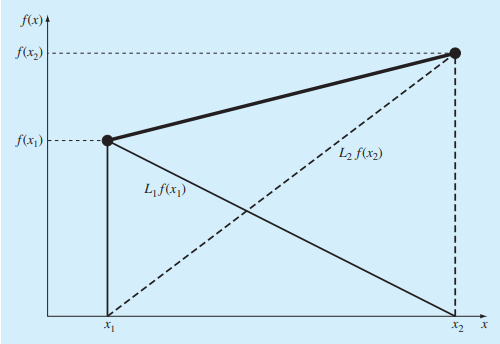
\includegraphics[scale=0.8]{fig_17_8}
   \caption{\textsf{A visual depiction of the rationale behind Lagrange interpolating polynomials. The figure shows
   the first-order case. Each of the two terms of Eq. (17.20) passes through one of the points and
   is zero at the other. The summation of the two terms must, therefore, be the unique straight line
   that connects the two points.}}\label{fig:fig_17_8}
\end{figure}

where
\begin{equation}
    \tag{17.23}
L_{i}(x)=\prod_{\substack{j=1 \\ j \neq i}}^{n} \frac{x-x_{j}}{x_{i}-x_{j}}
\end{equation}
where $n=$ the number of data points and $\prod$ designates the "product of."

\begin{exmp} \textbf{Lagrange Interpolating Polynomial}
    \noindent\textit{Problem Statement.}Use a Lagrange interpolating polynomial of the first and second
    order to evaluate the density of unused motor oil at T = 15 °C based on the following data:
    $$
\begin{array}{ll}
x_{1}=0 & f\left(x_{1}\right)=3.85 \\
x_{2}=20 & f\left(x_{2}\right)=0.800 \\
x_{3}=40 & f\left(x_{3}\right)=0.212
\end{array}
$$

    \noindent \textbf{Solution.} The first-order polynomial [Eq. (17.20)] can be used to obtain the estimate at $x=15$ :
    $$
    f_{1}(x)=\frac{15-20}{0-20} 3.85+\frac{15-0}{20-0} 0.800=1.5625
    $$
    In a similar fashion, the second-order polynomial is developed as [Eq. (17.21)]
    $$
    \begin{aligned}
    f_{2}(x)=& \frac{(15-20)(15-40)}{(0-20)(0-40)} 3.85+\frac{(15-0)(15-40)}{(20-0)(20-40)} 0.800 \\
    &+\frac{(15-0)(15-20)}{(40-0)(40-20)} 0.212=1.3316875
    \end{aligned}
    $$
\end{exmp}

\subsection{MATLAB M-file: Lagrange}
It is straightforward to develop an M-file based on Eqs. (17.22) and (17.23). As in
Fig. 17.9, the function is passed two vectors containing the independent (x) and the
dependent (y) variables. It is also passed the value of the independent variable where you
want to interpolate (xx). The order of the polynomial is based on the length of the x vector
that is passed. If n values are passed, an (n - 1)th order polynomial is fit. 

\begin{figure}[H]
    \centering
    
\includegraphics[scale=0.8]{fig_17_9}
   \caption{\textsf{An M-file to implement Lagrange interpolation.}}\label{fig:fig_17_9}
\end{figure}

\begin{lstlisting}[numbers=none]
    function yint = Lagrange(x,y,xx)
    % Lagrange: Lagrange interpolating polynomial
    %   yint = Lagrange(x,y,xx): Uses an (n - 1)-order
    %       Lagrange interpolating polynomial based on n data points
    %       to determine a value of the dependent variable (yint) at
    %       a given value of the independent variable, xx.
    % input:
    %   x = independent variable
    %   y = dependent variable
    %   xx = value of independent variable at which the
    %       interpolation is calculated
    % output:
    %   yint = interpolated value of dependent variable

    n = length(x);
    if length(y)~=n, error('x and y must be same length'); end
    s = 0;
    for i = 1:n
        product = y(i);
        for j = 1:n
            if i ~= j
                product = product*(xx-x(j))/(x(i)-x(j));
            end
        end
        s = s+product;
    end
    yint = s;
\end{lstlisting}

An example of a session using the function would be to predict the density of air at
1 atm pressure at a temperature of 15 °C based on the first four values from Table 17.1.
Because four values are passed to the function, a third-order polynomial would be implemented by the $Lagrange$ function to give:

\begin{lstlisting}[numbers=none]
>> format long
>> T = [-40 0 20 50];
>> d = [1.52 1.29 1.2 1.09];
>> density = Lagrange(T,d,15)
density =
    1.22112847222222
\end{lstlisting}

\noindent\textit{INVERSE INTERPOLATION}

As the nomenclature implies, the f (x) and x values in most interpolation contexts are the
dependent and independent variables, respectively. As a consequence, the values of the x's
are typically uniformly spaced. A simple example is a table of values derived for the function
f (x) = 1/x :
\begin{center}
\begin{tabular}{lccccccc}
    \hline $\boldsymbol{x}$ & 1 & 2 & 3 & 4 & 5 & 6 & 7 \\
    $\boldsymbol{f}(\boldsymbol{x})$ & 1 & $0.5$ & $0.3333$ & $0.25$ & $0.2$ & $0.1667$ & $0.1429$ \\
    \hline
    \end{tabular}
\end{center}
    Now suppose that you must use the same data, but you are given a value for $f(x)$ and must determine the corresponding value of $x$. For instance, for the data above, suppose that you were asked to determine the value of $x$ that corresponded to $f(x)=0.3$. For this case, because the function is available and easy to manipulate, the correct answer can be determined directly as $x=1 / 0.3=3.3333$.
    
    Such a problem is called inverse interpolation. For a more complicated case, you might be tempted to switch the $f(x)$ and $x$ values [i.e., merely plot $x$ versus $f(x)$ ] and use an approach like Newton or Lagrange interpolation to determine the result. Unfortunately, when you reverse the variables, there is no guarantee that the values along the new abscissa [the $f(x)$ 's] will be evenly spaced. In fact, in many cases, the values will be "telescoped." That is, they will have the appearance of a logarithmic scale with some adjacent points bunched together and others spread out widely. For example, for $f(x)=1 / x$ the result is
    \begin{center}
    \begin{tabular}{lccccccc}
    \hline $\boldsymbol{f}(\boldsymbol{x})$ & $0.1429$ & $0.1667$ & $0.2$ & $0.25$ & $0.3333$ & $0.5$ & 1 \\
    $\boldsymbol{x}$ & 7 & 6 & 5 & 4 & 3 & 2 & 1 \\
    \hline
    \end{tabular}
\end{center}
    Such nonuniform spacing on the abscissa often leads to oscillations in the resulting interpolating polynomial. This can occur even for lower-order polynomials. An alternative strategy is to fit an $n$ th-order interpolating polynomial, $f_{n}(x)$, to the original data [i.e., with $f(x)$ versus $x]$. In most cases, because the $x$ 's are evenly spaced, this polynomial will not be ill-conditioned. The answer to your problem then amounts to finding the value of $x$ that makes this polynomial equal to the given $f(x)$. Thus, the interpolation problem reduces to a roots problem!

    For example, for the problem just outlined, a simple approach would be to fit a quadratic polynomial to the three points: $(2,0.5),(3,0.3333)$, and $(4,0.25)$. The result would be
    $$
    f_{2}(x)=0.041667 x^{2}-0.375 x+1.08333
    $$
    The answer to the inverse interpolation problem of finding the $x$ corresponding to $f(x)=0.3$ would therefore involve determining the root of
    $$
    0.3=0.041667 x^{2}-0.375 x+1.08333
    $$
    For this simple case, the quadratic formula can be used to calculate
    $$
    x=\frac{0.375 \pm \sqrt{(-0.375)^{2}-4(0.041667) 0.78333}}{2(0.041667)}=\begin{aligned}
    &5.704158 \\
    &3.295842
    \end{aligned}
    $$
    Thus, the second root, $3.296$, is a good approximation of the true value of $3.333$. If additional accuracy were desired, a third- or fourth-order polynomial along with one of the root-location methods from Chaps. 5 or 6 could be employed.

    \section{EXTRAPOLATION AND OSCILLATIONS}
    Before leaving this chapter, there are two issues related to polynomial interpolation that
    must be addressed. These are extrapolation and oscillations.
    \subsection{Extrapolation}
    Extrapolation is the process of estimating a value of $f(x)$ that lies outside the range of the known base points, $x_{1}, x_{2}, \ldots, x_{n}$. As depicted in Fig. 17.10, the open-ended nature of

    \begin{figure}[H]
        \centering
        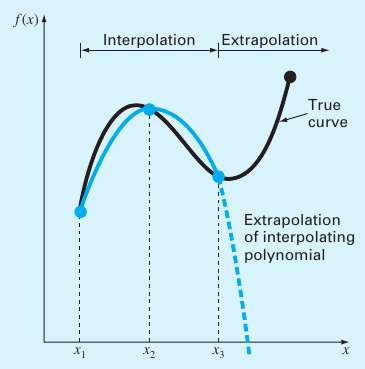
\includegraphics[scale=0.8]{fig_17_10}
       \caption{\textsf{Illustration of the possible divergence of an extrapolated prediction. The extrapolation is based
       on fitting a parabola through the first three known points.}}\label{fig:fig_17_10}
    \end{figure}
    extrapolation represents a step into the unknown because the process extends the curve
    beyond the known region. As such, the true curve could easily diverge from the prediction.
    Extreme care should, therefore, be exercised whenever a case arises where one must
    extrapolate.
    \begin{exmp} \textbf{Dangers of Extrapolation}
        \noindent\textit{Problem Statement.}
        This example is patterned after one originally developed by Forsythe,
        Malcolm, and Moler. The population in millions of the United States from 1920 to 2000 can
        be tabulated as
        $$
        \begin{array}{lccccccccc}
            \hline \text { Dafe } & 1920 & 1930 & 1940 & 1950 & 1960 & 1970 & 1980 & 1990 & 2000 \\
            \text { Population } & 106.46 & 123.08 & 132.12 & 152.27 & 180.67 & 205.05 & 227.23 & 249.46 & 281.42 \\
            \hline
            \end{array}
        $$
            Fit a seventh-order polynomial to the first 8 points (1920 to 1990). Use it to compute the
            population in 2000 by extrapolation and compare your prediction with the actual result.\\
        \noindent \textbf{Solution.} First, the data can be entered as

        \begin{lstlisting}[numbers=none]
>> t = [1920:10:1990];
>> pop = [106.46 123.08 132.12 152.27 180.67 205.05 227.23
249.46];
        \end{lstlisting}
        The $polyfit$ function can be used to compute the coefficients
        \begin{lstlisting}[numbers=none]
>> p = polyfit(t,pop,7)
        \end{lstlisting}
The polyfit function can be used to compute the coefficients
        \begin{lstlisting}[numbers=none]
Warning: Polynomial is badly conditioned. Remove repeated data
    points or try centering and scaling as described in HELP
    POLYFIT.
        \end{lstlisting}
        We can follow MATLAB's suggestion by scaling and centering the data values as in
        \begin{lstlisting}[numbers=none]
>> ts = (t - 1955)/35;
        \end{lstlisting}
        Now $polyfit$ works without an error message:
        \begin{lstlisting}[numbers=none]
>> p = polyfit(ts,pop,7);
        \end{lstlisting}
        We can then use the polynomial coefficients along with the polyval function to predict
the population in 2000 as
        \begin{lstlisting}[numbers=none]
>> polyval(p,(2000-1955)/35)
ans =
    175.0800
        \end{lstlisting}
        which is much lower that the true value of 281.42. Insight into the problem can be gained
by generating a plot of the data and the polynomial,
        \begin{lstlisting}[numbers=none]
>> tt = linspace(1920,2000);
>> pp = polyval(p,(tt-1955)/35);
>> plot(t,pop,'o',tt,pp)
        \end{lstlisting}

        \begin{figure}[H]
            \centering
            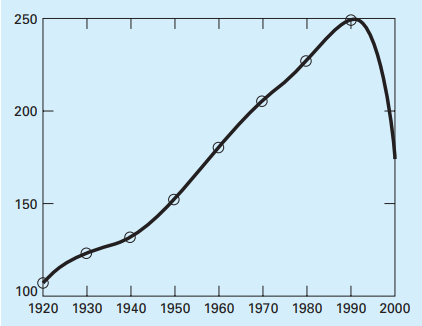
\includegraphics[scale=0.8]{fig_17_11}
           \caption{\textsf{Use of a seventh-order polynomial to make a prediction of U.S. population in 2000 based on
data from 1920 through 1990..}}\label{fig:fig_17_11}
        \end{figure}
        As in Fig. 17.11, the result indicates that the polynomial seems to fit the data nicely
        from 1920 to 1990. However, once we move beyond the range of the data into the realm of
        extrapolation, the seventh-order polynomial plunges to the erroneous prediction in 2000.
    \end{exmp}

\subsection{Oscillations}

Although “more is better” in many contexts, it is absolutely not true for polynomial interpolation. Higher-order polynomials tend to be very ill-conditioned—that is, they tend to be
highly sensitive to round-off error. The following example illustrates this point nicely.

\begin{exmp} \textbf{Dangers of Higher-Order Polynomial Interpolation}
    \noindent\textit{Problem Statement.} In 1901, Carl Runge published a study on the dangers of higherorder polynomial interpolation. He looked at the following simple-looking function:
    \begin{equation}
        \tag{17.24}
        f(x)=\frac{1}{1+25 x^{2}}
        \end{equation}
        which is now called Runge's function. He took equidistantly spaced data points from this
        function over the interval [-1, 1]. He then used interpolating polynomials of increasing
        order and found that as he took more points, the polynomials and the original curve differed
        considerably. Further, the situation deteriorated greatly as the order was increased. Duplicate Runge's result by using the polyfit and polyval functions to fit fourth- and tenthorder polynomials to 5 and 11 equally spaced points generated with Eq. (17.24). Create
        plots of your results along with the sampled values and the complete Runge's function.\\

    \noindent \textbf{Solution.} The five equally spaced data points can be generated as in
    \begin{lstlisting}[numbers=none]
>> x = linspace(-1,1,5);
>> y = 1./(1+25*x.^2);
    \end{lstlisting}
    Next, a more finally spaced vector of xx values can be computed so that we can create a
smooth plot of the results:
    \begin{lstlisting}[numbers=none]
>> xx = linspace(-1,1);
    \end{lstlisting}
    Recall that $linspace$ automatically creates 100 points if the desired number of points is
not specified. The $polyfit$ function can be used to generate the coefficients of the fourthorder polynomial, and the $polval$ function can be used to generate the polynomial interpolation at the finely spaced values of xx:

    \begin{lstlisting}[numbers=none]
>> p = polyfit(x,y,4);
>> y4 = polyval(p,xx);
    \end{lstlisting}
    Finally, we can generate values for Runge's function itself and plot them along with the
polynomial fit and the sampled data:
    \begin{lstlisting}[numbers=none]
>> yr = 1./(1+25*xx.^2);
>> plot(x,y,'o',xx,y4,xx,yr,'--')
    \end{lstlisting}
    As in Fig. 17.12, the polynomial does a poor job of following Runge's function\\
    Continuing with the analysis, the tenth-order polynomial can be generated and plotted
with
    \begin{lstlisting}[numbers=none]
>> x = linspace(-1,1,11);
>> y = 1./(1+25*x.^2);
    \end{lstlisting}

    \begin{figure}[H]
        \centering
        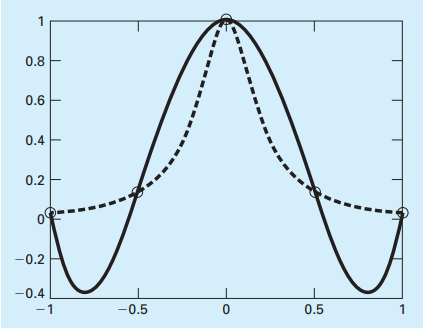
\includegraphics[scale=0.8]{fig_17_12}
       \caption{\textsf{Comparison of Runge's function (dashed line) with a fourth-order polynomial fit to 5 points
       sampled from the function.}}\label{fig:fig_17_12}
    \end{figure}
    \begin{figure}[H]
        \centering
        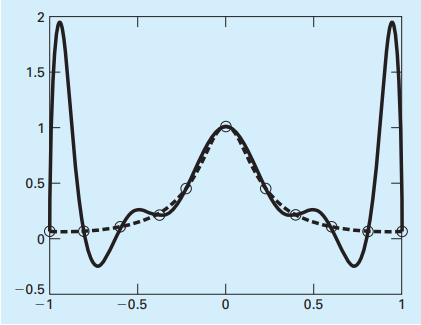
\includegraphics[scale=0.8]{fig_17_13}
       \caption{\textsf{Comparison of Runge's function (dashed line) with a tenth-order polynomial fit to 11 points
       sampled from the function.}}\label{fig:fig_17_13}
    \end{figure}
    \begin{lstlisting}[numbers=none]
>> p = polyfit(x,y,10);
>> y10 = polyval(p,xx);
>> plot(x,y,'o',xx,y10,xx,yr,'--')
    \end{lstlisting}
    As in Fig. 17.13, the fit has gotten even worse, particularly at the ends of the interval!\\
    Although there may be certain contexts where higher-order polynomials are necessary,
they are usually to be avoided. In most engineering and scientific contexts, lower-order
polynomials of the type described in this chapter can be used effectively to capture the
curving trends of data without suffering from oscillations.
\end{exmp}


\section*{PROBLEMS}
\begin{multicols}{2}

\noindent\textit{17.1} The following data come from a table that was measured with high precision. Use the best numerical method
(for this type of problem) to determine y at x = 3.5. Note
that a polynomial will yield an exact value. Your solution
should prove that your result is exact.

$$
\begin{array}{cccccccc}
\hline \boldsymbol{x} & 0 & 1.8 & 5 & 6 & 8.2 & 9.2 & 12 \\
\boldsymbol{y} & 26 & 16.415 & 5.375 & 3.5 & 2.015 & 2.54 & 8 \\
\hline
\end{array}
$$

\noindent\textit{17.2} Use Newton's interpolating polynomial to determine y at
x = 3.5 to the best possible accuracy. Compute the finite divided differences as in Fig. 17.5, and order your points to attain
optimal accuracy and convergence. That is, the points should
be centered around and as close as possible to the unknown.

$$
\begin{array}{cccccccc}
\hline \boldsymbol{x} & 0 & 1 & 2.5 & 3 & 4.5 & 5 & 6 \\
\boldsymbol{y} & 2 & 5.4375 & 7.3516 & 7.5625 & 8.4453 & 9.1875 & 12 \\
\hline
\end{array}
$$

\noindent\textit{17.3} Use Newton's interpolating polynomial to determine y at
x = 8 to the best possible accuracy. Compute the finite divided
differences as in Fig. 17.5, and order your points to attain optimal accuracy and convergence. That is, the points should be
centered around and as close as possible to the unknown.

$$
\begin{array}{ccccccccc}
\hline \boldsymbol{x} & 0 & 1 & 2 & 5.5 & 11 & 13 & 16 & 18 \\
\boldsymbol{y} & 0.5 & 3.134 & 5.3 & 9.9 & 10.2 & 9.35 & 7.2 & 6.2 \\
\hline
\end{array}
$$

\noindent\textit{17.4} Given the data

$$
\begin{array}{lllllll}
\hline \boldsymbol{x} & 1 & 2 & 2.5 & 3 & 4 & 5 \\
\boldsymbol{f}(\boldsymbol{x}) & 0 & 5 & 6.5 & 7 & 3 & 1 \\
\hline
\end{array}
$$

(a) Calculate f (3.4) using Newton's interpolating polynomials of order 1 through 3. Choose the sequence of the points
for your estimates to attain the best possible accuracy.
That is, the points should be centered around and as close
as possible to the unknown.\\
(b) Repeat (a) but use the Lagrange polynomial.

\noindent\textit{17.5} Given the data

$$
\begin{array}{lccccc}
\hline \boldsymbol{x} & 1 & 2 & 3 & 5 & 6 \\
f(x) & 7 & 4 & 5.5 & 40 & 82 \\
\hline
\end{array}
$$
Calculate f (4) using Newton's interpolating polynomials of
order 1 through 4. Choose your base points to attain good
accuracy. That is, the points should be centered around and
as close as possible to the unknown. What do your results
indicate regarding the order of the polynomial used to generate the data in the table?

\noindent\textit{17.6}
Repeat Prob. 17.5 using the Lagrange polynomial of
order 1 through 3.\\
\noindent\textit{17.7}
Table P15.5 lists values for dissolved oxygen concentration in water as a function of temperature and chloride
concentration.\\
(a) Use quadratic and cubic interpolation to determine the
oxygen concentration for T = 12 °C and c = 10 g/L.\\
(b) Use linear interpolation to determine the oxygen concentration for T = 12 °C and c = 15 g/L.\\
(c) Repeat (b) but use quadratic interpolation.

\noindent\textit{17.8} Employ inverse interpolation using a cubic interpolating polynomial and bisection to determine the value of x that
corresponds to f (x) = 1.7 for the following tabulated data:

$$
\begin{array}{lccccccc}
\hline \boldsymbol{x} & 1 & 2 & 3 & 4 & 5 & 6 & 7 \\
\boldsymbol{f}(\boldsymbol{x}) & 3.6 & 1.8 & 1.2 & 0.9 & 0.72 & 1.5 & 0.51429 \\
\hline
\end{array}
$$

\noindent\textit{17.9} Employ inverse interpolation to determine the value of
x that corresponds to f (x) = 0.93 for the following tabulated data:
$$
\begin{array}{lccccccc}
    \hline \boldsymbol{x} & 0 & 1 & 2 & 3 & 4 & 5 \\
    \boldsymbol{f}(\boldsymbol{x}) & 0 & 0.5 & 0.8 & 0.9 & 0.941176 & 0.961538 \\
    \hline
\end{array}
$$
    Note that the values in the table were generated with the function $f(x)=x^{2} /\left(1+x^{2}\right)$.
    (a) Determine the correct value analytically.\\
    (b) Use quadratic interpolation and the quadratic formula to
    determine the value numerically.\\
    (c) Use cubic interpolation and bisection to determine the
    value numerically.\\
    \noindent\textit{17.10} Use the portion of the given steam table for superheated water at 200 MPa to find (a) the corresponding
    entropy s for a specific volume v of 0.118 with linear interpolation, (b) the same corresponding entropy using quadratic interpolation, and (c) the volume corresponding to an
    entropy of 6.45 using inverse interpolation.
    $$
    \begin{array}{llll}
    \hline \boldsymbol{v}, \mathbf{m}^{\mathbf{3}} / \mathbf{k g} & 0.10377 & 0.11144 & 0.12547 \\
    \boldsymbol{s}, \mathbf{k} \mathbf{J} /(\mathbf{k g} \mathbf{K}) & 0.4147 & 0.5453 & 6.7664 \\
    \hline
    \end{array}
    $$

    \noindent\textit{17.11} The following data for the density of nitrogen gas versus temperature come from a table that was measured with
    high precision. Use first- through fifth-order polynomials to
    estimate the density at a temperature of 330 K. What is your
    best estimate? Employ this best estimate and inverse interpolation to determine the corresponding temperature.
    $$
    \begin{array}{lcccccc}
    \hline \boldsymbol{T}, \mathbf{K} & 200 & 250 & 300 & 350 & 400 & 450 \\
    \text { Density, } & 1.708 & 1.367 & 1.139 & 0.967 & 0.854 & 0.759 \\
    \mathbf{k g} / \mathbf{m}^{3} & & & & & & \\
    \hline
    \end{array}
    $$
    \noindent\textit{17.12} Ohm's law states that the voltage drop V across an
    ideal resistor is linearly proportional to the current i flowing
    through the resister as in V = i R, where R is the resistance.
    However, real resistors may not always obey Ohm's law.
    Suppose that you performed some very precise experiments
    to measure the voltage drop and corresponding current for a
    resistor. The following results suggest a curvilinear relationship rather than the straight line represented by Ohm's law:
    $$
    \begin{array}{lcccccc}
    \hline \boldsymbol{i} & -1 & -0.5 & -0.25 & 0.25 & 0.5 & 1 \\
    \boldsymbol{V} & -637 & -96.5 & -20.5 & 20.5 & 96.5 & 637 \\
    \hline
    \end{array}
    $$
    To quantify this relationship, a curve must be fit to the data. Because of measurement error, regression would typically be the
preferred method of curve fitting for analyzing such experimental data. However, the smoothness of the relationship, as
well as the precision of the experimental methods, suggests
that interpolation might be appropriate. Use a fifth-order interpolating polynomial to fit the data and compute V for i = 0.10.

\noindent\textit{17.13} Bessel functions often arise in advanced engineering
analyses such as the study of electric fields. Here are some
selected values for the zero-order Bessel function of the first
kind
$$
\begin{array}{lccccc}
\hline \boldsymbol{x} & 1.8 & 2.0 & 2.2 & 2.4 & 2.6 \\
\boldsymbol{J}_{1}(\boldsymbol{x}) & 0.5815 & 0.5767 & 0.5560 & 0.5202 & 0.4708 \\
\hline
\end{array}
$$
Estimate $J\textsubscript{1}$(2.1) using third- and fourth-order interpolating
polynomials. Determine the percent relative error for each
case based on the true value, which can be determined with
MATLAB's built-in function $besselj$.

\noindent\textit{17.14} 4 Repeat Example 17.6 but using first-, second-, third-,
and fourth-order interpolating polynomials to predict the
population in 2000 based on the most recent data. That is, for
the linear prediction use the data from 1980 and 1990, for the
quadratic prediction use the data from 1970, 1980, and 1990,
and so on. Which approach yields the best result?

\noindent\textit{17.15} The specific volume of a superheated steam is listed

in steam tables for various temperatures. For example, at a pressure of $3000 \mathrm{lb} / \mathrm{in}^{2}$, absolute:
\begin{tabular}{lccccc}
\hline $\boldsymbol{T},{ }^{\circ} \mathbf{C}$ & 370 & 382 & 394 & 406 & 418 \\
$\boldsymbol{v}_{\boldsymbol{,}} \mathbf{L t}^{\mathbf{3}} / \mathbf{k g}$ & $5.9313$ & $7.5838$ & $8.8428$ & $9.796$ & $10.5311$ \\
\hline
\end{tabular}
Determine v at T = 750 °F.\\

\noindent\textit{17.16} The vertical stress $\sigma_{z}$ under the corner of a rectangular area subjected to a uniform load of intensity $q$ is given by the solution of Boussinesq's equation:
$$
\begin{array}{r}
\sigma=\frac{q}{4 \pi}\left[\frac{2 m n \sqrt{m^{2}+n^{2}+1}}{m^{2}+n^{2}+1+m^{2} n^{2}} \frac{m^{2}+n^{2}+2}{m^{2}+n^{2}+1}\right. \\
\left.+\sin ^{-1}\left(\frac{2 m n \sqrt{m^{2}+n^{2}+1}}{m^{2}+n^{2}+1+m^{2} n^{2}}\right)\right]
\end{array}
$$
Because this equation is inconvenient to solve manually, it has been reformulated as
$$
\sigma_{z}=q f_{z}(m, n)
$$
where $f_{z}(m, n)$ is called the influence value, and $m$ and $n$ are dimensionless ratios, with $m=a / z$ and $n=b / z$ and $a$ and $b$ are defined in Fig. P17.16. The influence value is then tabulated, a portion of which is given in Table P17.16. If $a=4.6$ and $b=14$, use a third-order interpolating polynomial to compute $\sigma_{z}$ at a depth $10 \mathrm{~m}$ below the corner of a rectangular footing that is subject to a total load of $100 \mathrm{t}$
\begin{figure}[H]
    \centering
    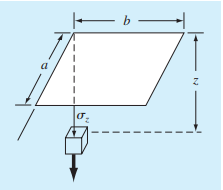
\includegraphics[scale=0.8]{fig_17_16}
   \caption{\textsf{}}\label{fig:fig_17_16}
\end{figure}
(metric tons). Express your answer in tonnes per square
meter. Note that q is equal to the load per area.

$$
\begin{array}{llll}
\hline \boldsymbol{m} & \boldsymbol{n}=\mathbf{1 . 2} & \boldsymbol{n}=\mathbf{1 . 4} & \boldsymbol{n}=\mathbf{1 . 6} \\
\hline 0.1 & 0.02926 & 0.03007 & 0.03058 \\
0.2 & 0.05733 & 0.05894 & 0.05994 \\
0.3 & 0.08323 & 0.08561 & 0.08709 \\
0.4 & 0.10631 & 0.10941 & 0.11135 \\
0.5 & 0.12626 & 0.13003 & 0.13241 \\
0.6 & 0.14309 & 0.14749 & 0.15027 \\
0.7 & 0.15703 & 0.16199 & 0.16515 \\
0.8 & 0.16843 & 0.17389 & 0.17739 \\
\hline\\
\end{array}
$$
\noindent\textit{TABLE P17.16}\\
\noindent\textit{17.17} You measure the voltage drop V across a resistor for a
number of different values of current i. The results are
$$
\begin{array}{lccccc}
\hline \boldsymbol{i} & 0.25 & 0.75 & 1.25 & 1.5 & 2.0 \\
\boldsymbol{V} & -0.45 & -0.6 & 0.70 & 1.88 & 6.0 \\
\hline \hline
\end{array}
$$
Use first- through fourth-order polynomial interpolation to
estimate the voltage drop for i = 1.15. Interpret your results.\\

\noindent\textit{17.18} The current in a wire is measured with great precision
as a function of time:
$$
\begin{array}{lccccc}
\hline \boldsymbol{t} & 0 & 0.1250 & 0.2500 & 0.3750 & 0.5000 \\
\boldsymbol{i} & 0 & 6.24 & 7.75 & 4.85 & 0.0000 \\
\hline
\end{array}
$$
Determine i at t = 0.23.\\

\noindent\textit{17.19} The acceleration due to gravity at an altitude y above
the surface of the earth is given by
$$
\begin{array}{lccccc}
\hline \boldsymbol{y}, \mathbf{m} & 0 & 30,000 & 60,000 & 90,000 & 120,000 \\
\boldsymbol{g}, \mathbf{m} / \mathbf{s}^{\mathbf{2}} & 9.8100 & 9.7487 & 9.6879 & 9.6278 & 9.5682 \\
\hline
\end{array}
$$
Compute g at y = 55,000 m.\\

\noindent\textit{17.20} Temperatures are measured at various points on a
heated plate (Table P17.20). Estimate the temperature at
(a) x = 4, y = 3.2, and (b) x = 4.3, y = 2.7.

$$
\begin{array}{lccccc}
\hline & \boldsymbol{x}=\mathbf{0} & \boldsymbol{x}=\mathbf{2} & \boldsymbol{x}=\mathbf{4} & \boldsymbol{x}=\mathbf{6} & \boldsymbol{x}=\mathbf{8} \\
\hline \boldsymbol{y} = \mathbf { 0 } & 100.00 & 90.00 & 80.00 & 70.00 & 60.00 \\
\boldsymbol{y}=\mathbf{2} & 85.00 & 64.49 & 53.50 & 48.15 & 50.00 \\
\boldsymbol{y}=\mathbf{4} & 70.00 & 48.90 & 38.43 & 35.03 & 40.00 \\
\boldsymbol{y}=\mathbf{6} & 55.00 & 38.78 & 30.39 & 27.07 & 30.00 \\
\boldsymbol{y}=\mathbf{8} & 40.00 & 35.00 & 30.00 & 25.00 & 20.00 \\
\hline
\end{array}
$$
\noindent\textit{TABLE P17.20} Temperatures (°C) at various points
on a square heated plate.

\noindent\textit{17.21}

Use the portion of the given steam table for superheated $H\textsubscript{2}O$ at 200 MPa to (a) find the corresponding
entropy s for a specific volume v of $\mathrm{m}^{3} / \mathrm{kg}$ with linear
interpolation, (b) find the same corresponding entropy using
quadratic interpolation, and (c) find the volume corresponding to an entropy of 6.6 using inverse interpolation.

$$
\begin{array}{lccc}
\hline \boldsymbol{v}\left(\mathbf{m}^{\mathbf{3}} / \mathbf{k g}\right) & 0.10377 & 0.11144 & 0.12540 \\
\boldsymbol{s}(\mathbf{k} \mathbf{J} / \mathbf{k g} \cdot \mathbf{K}) & 6.4147 & 6.5453 & 6.7664 \\
\hline
\end{array}
$$

\end{multicols}

\end{document}
\noindent\textit{17.2}
$x\textsubscript{1}$

\begin{equation}
    \tag{17.} \nonumber
    -
\end{equation}

\begin{lstlisting}[numbers=none]
\end{lstlisting}

\section{INTRODUCTION TO SPLINES}
\subsection{End Conditions}

\begin{figure}[H]
    \centering
    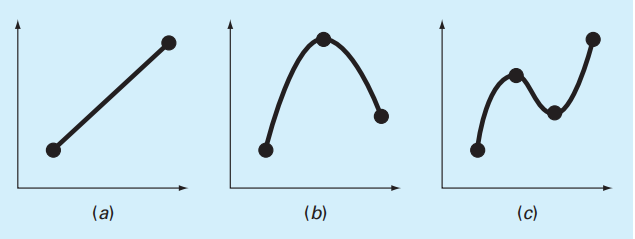
\includegraphics[scale=0.8]{fig_17_1}
   \caption{\textsf{}}\label{fig:fig_17_}
\end{figure}

\begin{exmp} \textbf{First-Order Splines}
    \noindent\textit{Problem Statement.}
    \noindent \textbf{Solution.}
\end{exmp}